% Página
\section{Segurança das Chaves de Criptografia}

\subsection{Alice}

Processo de criação das chaves, Pública (KPuAlice.pem), Privada (KPrAlice.pem) e de Dados (DEKAlice.bin), juntamente com o processo de encriptação para armazenamento seguro das chaves Privada (KPrAlice.pem) e de Dados (DEKAlice).

\begin{figure}[H]
	\centering
	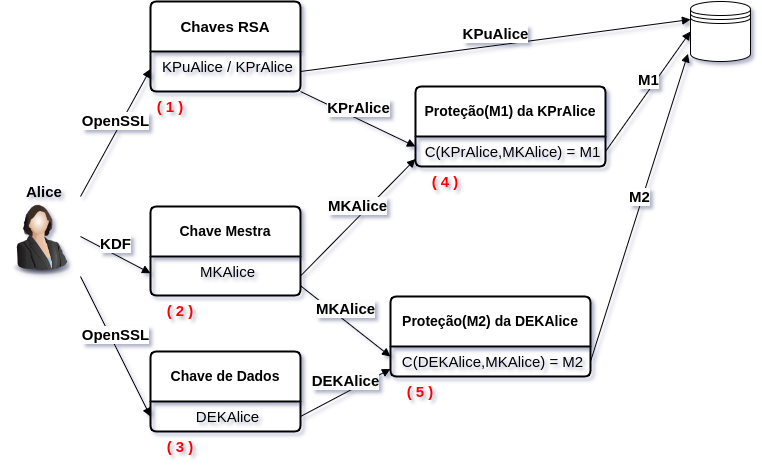
\includegraphics[scale=0.55]{chave_alice.png}
	\caption{Chaves e Processos associadas a Alice (M1 e M2: ver nota sobre autenticação)}
	\label{fig:chave_alice}
\end{figure}

\begin{enumerate}
	\item Criação da Chave Pública (KPuAlice.pem) e da Chave Privada (KPrAlice.pem);
	\begin{tcolorbox}[width=\textwidth]
		{\scriptsize
			\begin{verbatim}
			$ openssl genpkey -algorithm RSA -pkeyopt rsa_keygen_bits:2048 -out KPrAlice.pem
			$ openssl rsa -pubout -in KPrAlice.pem -out KPuAlice.pem
			$ openssl req -new -x509 -key KPrAlice.pem -out Alice.cert.pem \
			  -subj "/CN=Alice"
			\end{verbatim}
		}
	\end{tcolorbox}
	\item Derivação local da Chave Mestra da Alice (MKAlice.hex), baseada na Senha Mestra (MPAlice). O salt de 128 bits é armazenado separadamente para permitir a derivação durante a recuperação;
	\begin{tcolorbox}[width=\textwidth]
		{\scriptsize
			\begin{verbatim}
			$ read -rs MASTER_PASSWORD
			$ SALT_HEX=$(openssl rand -hex 16)
			$ printf '%s' "$SALT_HEX" > MKAlice.salt
			$ openssl kdf -keylen 32 -kdfopt digest:SHA256 \
			  -kdfopt pass:"$MASTER_PASSWORD" -kdfopt salt:"$SALT_HEX" \
			  -kdfopt iter:600000 PBKDF2 | tr -d ':\n' > MKAlice.hex
			\end{verbatim}
		}
	\end{tcolorbox}
	\item Criação da Chave de Dados (DEKAlice.bin);
	\begin{tcolorbox}[width=\textwidth]
		{\scriptsize
			\begin{verbatim}
			$ openssl rand -out DEKAlice.bin 32
			\end{verbatim}
		}
	\end{tcolorbox}
	\item A Chave Privada (KPrAlice.pem) é protegida com a Chave Mestra (MKAlice.hex), gerando o Texto Cifrado M1. O IV é armazenado junto com o artefato cifrado;
	\begin{tcolorbox}[width=\textwidth]
		{\scriptsize
			\begin{verbatim}
			$ IV_HEX=$(openssl rand -hex 16)
			$ printf '%s' "$IV_HEX" > M1.iv
			$ openssl enc -aes-256-cbc -K "$(cat MKAlice.hex)" -iv "$IV_HEX" \
			  -in KPrAlice.pem -out M1.bin
			\end{verbatim}
		}
	\end{tcolorbox}
	\item A Chave de Dados (DEKAlice.bin) é protegida com a Chave Mestra (MKAlice.hex), gerando o Texto Cifrado M2 que é enviado para o servidor.
	\begin{tcolorbox}[width=\textwidth]
		{\scriptsize
			\begin{verbatim}
			$ IV_HEX=$(openssl rand -hex 16)
			$ printf '%s' "$IV_HEX" > M2.iv
			$ openssl enc -aes-256-cbc -K "$(cat MKAlice.hex)" -iv "$IV_HEX" \
			  -in DEKAlice.bin -out M2.bin
			\end{verbatim}
		}
	\end{tcolorbox}
\end{enumerate}

\subsection{Bob}

Processo de criação das chaves, Pública (KPuBob.pem), Privada (KPrBob.pem) e de Dados (DEKBob.bin), juntamente com o processo de encriptação para armazenamento seguro das chaves Privada (KPrBob.pem) e de Dados (DEKBob.bin).

\begin{figure}[H]
	\centering
	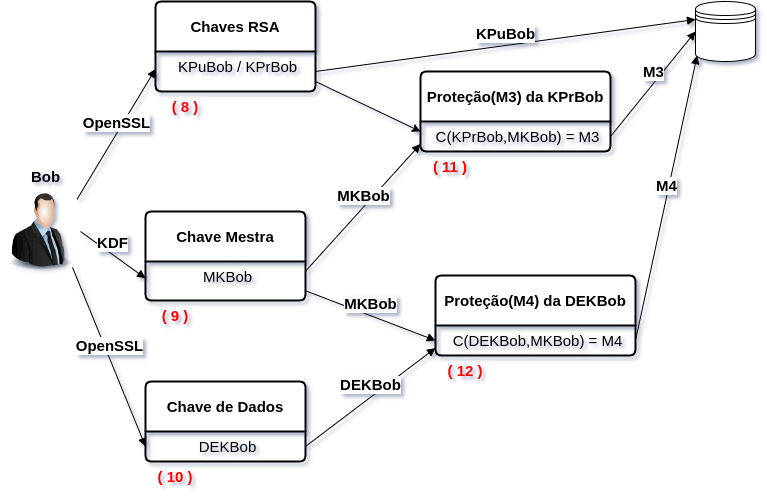
\includegraphics[scale=0.55]{chave_bob.png}
	\caption{Chaves e Processos associados ao Bob (M3 e M4: ver nota sobre autenticação)}
	\label{fig:chave_bob}
\end{figure}

\begin{enumerate}
	\setcounter{enumi}{7} % Define o contador para começar do número 8
		\item Criação das Chave Pública (KPuBob.pem) e da Chave Privada (KPrBob.pem);
		\begin{tcolorbox}[width=\textwidth]
			{\scriptsize
				\begin{verbatim}
				$ openssl genpkey -algorithm RSA -pkeyopt rsa_keygen_bits:2048 -out KPrBob.pem
				$ openssl rsa -pubout -in KPrBob.pem -out KPuBob.pem
				\end{verbatim}
			}
		\end{tcolorbox}
		\item Derivação local da Chave Mestra (MKBob.hex) baseada na Senha Mestra (MPBob);
		\begin{tcolorbox}[width=\textwidth]
			{\scriptsize
				\begin{verbatim}
					$ read -rs MASTER_PASSWORD
					$ SALT_HEX=$(openssl rand -hex 16)
					$ printf '%s' "$SALT_HEX" > MKBob.salt
					$ openssl kdf -keylen 32 -kdfopt digest:SHA256 \
					  -kdfopt pass:"$MASTER_PASSWORD" -kdfopt salt:"$SALT_HEX" \
					  -kdfopt iter:600000 PBKDF2 | tr -d ':\n' > MKBob.hex
				\end{verbatim}
			}
		\end{tcolorbox}
		\item Criação da Chave de Dados (DEKBob.bin);
		\begin{tcolorbox}[width=\textwidth]
			{\scriptsize
				\begin{verbatim}
				$ openssl rand -out DEKBob.bin 32
				\end{verbatim}
			}
		\end{tcolorbox}
		\item A Chave Privada (KPrBob) é protegida com a Chave Mestra (MKBob.hex), gerando o Texto Cifrado M3 que é enviado para o servidor;
		\begin{tcolorbox}[width=\textwidth]
			{\scriptsize
				\begin{verbatim}
				$ IV_HEX=$(openssl rand -hex 16)
				$ printf '%s' "$IV_HEX" > M3.iv
				$ openssl enc -aes-256-cbc -K "$(cat MKBob.hex)" -iv "$IV_HEX" \
				  -in KPrBob.pem -out M3.bin
				\end{verbatim}
			}
		\end{tcolorbox}
		\item A Chave de Dados (DEKBob.bin) é protegida com a Chave Mestra (MKBob.hex), gerando o Texto Cifrado M4 que é enviado para o servidor.
		\begin{tcolorbox}[width=\textwidth]
			{\scriptsize
				\begin{verbatim}
				$ IV_HEX=$(openssl rand -hex 16)
				$ printf '%s' "$IV_HEX" > M4.iv
				$ openssl enc -aes-256-cbc -K "$(cat MKBob.hex)" -iv "$IV_HEX" \
				  -in DEKBob.bin -out M4.bin
				\end{verbatim}
			}
		\end{tcolorbox}
\end{enumerate}

\pagebreak
